% This must be in the first 5 lines to tell arXiv to use pdfLaTeX, which is strongly recommended.
\pdfoutput=1
% In particular, the hyperref package requires pdfLaTeX in order to break URLs across lines.

\documentclass[11pt]{article}
\usepackage[margin=1in]{geometry}
% Change "review" to "final" to generate the final (sometimes called camera-ready) version.
% Change to "preprint" to generate a non-anonymous version with page numbers.
\usepackage[review]{acl}

% Standard package includes
\usepackage{times}
\usepackage{latexsym}

% For proper rendering and hyphenation of words containing Latin characters (including in bib files)
\usepackage[T1]{fontenc}
% For Vietnamese characters
% \usepackage[T5]{fontenc}
% See https://www.latex-project.org/help/documentation/encguide.pdf for other character sets

% This assumes your files are encoded as UTF8
\usepackage[utf8]{inputenc}

% This is not strictly necessary, and may be commented out,
% but it will improve the layout of the manuscript,
% and will typically save some space.
\usepackage{microtype}

% This is also not strictly necessary, and may be commented out.
% However, it will improve the aesthetics of text in
% the typewriter font.
\usepackage{inconsolata}

%Including images in your LaTeX document requires adding
%additional package(s)
\usepackage{graphicx}

\usepackage{longtable}
\usepackage{booktabs}
\usepackage{amsmath} 
\usepackage{natbib}

% If the title and author information does not fit in the area allocated, uncomment the following
%
%\setlength\titlebox{<dim>}
%
% and set <dim> to something 5cm or larger.

\title{A Stylometric Application of Large Language Models}

% Author information can be set in various styles:
% For several authors from the same institution:
% \author{Author 1 \and ... \and Author n \\
%         Address line \\ ... \\ Address line}
% if the names do not fit well on one line use
%         Author 1 \\ {\bf Author 2} \\ ... \\ {\bf Author n} \\
% For authors from different institutions:
% \author{Author 1 \\ Address line \\  ... \\ Address line
%         \And  ... \And
%         Author n \\ Address line \\ ... \\ Address line}
% To start a separate ``row'' of authors use \AND, as in
% \author{Author 1 \\ Address line \\  ... \\ Address line
%         \AND
%         Author 2 \\ Address line \\ ... \\ Address line \And
%         Author 3 \\ Address line \\ ... \\ Address line}

% \author{First Author \\
%   Affiliation / Address line 1 \\
%   Affiliation / Address line 2 \\
%   Affiliation / Address line 3 \\
%   \texttt{email@domain} \\\And
%   Second Author \\
%   Affiliation / Address line 1 \\
%   Affiliation / Address line 2 \\
%   Affiliation / Address line 3 \\
%   \texttt{email@domain} \\}

%\author{
%  \textbf{First Author\textsuperscript{1}},
%  \textbf{Second Author\textsuperscript{1,2}},
%  \textbf{Third T. Author\textsuperscript{1}},
%  \textbf{Fourth Author\textsuperscript{1}},
%\\
%  \textbf{Fifth Author\textsuperscript{1,2}},
%  \textbf{Sixth Author\textsuperscript{1}},
%  \textbf{Seventh Author\textsuperscript{1}},
%  \textbf{Eighth Author \textsuperscript{1,2,3,4}},
%\\
%  \textbf{Ninth Author\textsuperscript{1}},
%  \textbf{Tenth Author\textsuperscript{1}},
%  \textbf{Eleventh E. Author\textsuperscript{1,2,3,4,5}},
%  \textbf{Twelfth Author\textsuperscript{1}},
%\\
%  \textbf{Thirteenth Author\textsuperscript{3}},
%  \textbf{Fourteenth F. Author\textsuperscript{2,4}},
%  \textbf{Fifteenth Author\textsuperscript{1}},
%  \textbf{Sixteenth Author\textsuperscript{1}},
%\\
%  \textbf{Seventeenth S. Author\textsuperscript{4,5}},
%  \textbf{Eighteenth Author\textsuperscript{3,4}},
%  \textbf{Nineteenth N. Author\textsuperscript{2,5}},
%  \textbf{Twentieth Author\textsuperscript{1}}
%\\
%\\
%  \textsuperscript{1}Affiliation 1,
%  \textsuperscript{2}Affiliation 2,
%  \textsuperscript{3}Affiliation 3,
%  \textsuperscript{4}Affiliation 4,
%  \textsuperscript{5}Affiliation 5
%\\
%  \small{
%    \textbf{Correspondence:} \href{mailto:email@domain}{email@domain}
%  }
%}

\begin{document}
\maketitle
\begin{abstract}

Stylometry is the quantitative analysis of writing style. In this paper we show
that large language models can be used to distinguish the writings of different
authors. Specifically, an individual model, trained on the works of one author,
will predict held-out text from that author more accurately than held-out text
from other authors. We suggest that, in this way, a model trained on one
author's works embodies the unique writing style of that author. In our primary
example, we use this approach to confirm R. P. Thompson's authorship of the
well-studied 15th book of the ``Oz'' series, originally attributed to F. L.
Baum. We also include other (known) authorship comparison pairs.

\end{abstract}

\section{Introduction}

The quantitative measure of writing style --- stylometry --- has a long
history, and generally elides the complex collection of factors that may go
into an author's ``voice'', focusing instead on statistics derived from the
text~\citep{NealEtal17}. In literature, ``style" refers to the distinctive
manner in which language is used. It encompasses choices in vocabulary,
sentence structure, tone, and the use of rhetorical devices. Style is distinct
from semantics, which is concerned with the meaning and interpretation of text.
In brief, content is what you say, and style is the way you say it. Many mark
the birth of the subject with the late nineteenth century work of the
philologist Wincenty Lutos{\l}awski, who had an interest in finding a
statistical basis for addressing a long-standing problem in Classics of
estimating the temporal order of Plato's Dialogues~\citep{Howl91}. Toward this
end, Lutos{\l}awski measured hundreds of variables to arrive at his
conclusions~\citep{Luto97}.

An ability to quantify authorial voice is also useful for authorship
attribution and is perhaps the most common application of stylometric
techniques~\citep{Juol08}. Among the most famous results to date is Mosteller
and Wallace's work on determining the authorship of The Federalist Papers,
eighty-five essays in support of ratification of the Constitution, authored by
the anonymous ``Publius" over 1787-1788, but known to have been (individually)
written by John Jay, James Madison, and Alexander Hamilton. Mosteller and
Wallace used Bayesian techniques directed at simple word frequency statistics
to hypothesize attribution of the essays, and their results are generally
accepted by domain experts in political history~\citep{MostWall63, MostWall84}.
Other approaches of note work with feature vectors whose entries record word
frequencies in the texts, with works of known attribution giving ground-truth
and disputed attributions resolved according to their similarity to the known.
The words under consideration are picked according to a range of criteria. A
common choice is the use of function words\footnote{``Function words" are words
that have no particular contextual information (e.g., prepositions, articles,
conjunctions).} used to build a simple classifier with feature vectors of word
frequencies~\citep{NiloEtal99}. Famously, this was used to help settle
uncertainty around the authorship of the 15\textsuperscript{th} book in the 31
book \emph{Oz} series~\citep{NiloBino03}. In~\citet{HughEtal12}, feature
vectors constructed from the frequencies of function words are used to show
evidence for an evolutionary pattern of writing style in the text corpus
comprised by the Gutenberg.org collection. See \citet{NealEtal17} for a
relatively recent survey of stylometric techniques. More generally, stylometric
analysis is among the techniques available to those whose work engages with the
practice of ``distant reading"~\citep{More17, More00} (the machine reading of
text at large scales) which is a part of the broader digital humanities and the
practices of cultural analytics.


\section{Methods}

In this section, we outline our methodology for identifying stylometric
signatures using large language models. For each selected author, we train a
GPT-2 model on that author's corpus. We then use the trained model to compute
the prediction loss on some held-out texts from both the target author and
other authors in the dataset. By comparing these losses, we assess whether the
model captures author-specific stylistic patterns: a model trained on a given
author should exhibit lower loss when predicting that author's own texts
compared to those of others.

We begin by applying this approach to compare the works of Thompson and Baum,
both authors of books in the \emph{Oz} series. We then extend our analysis to a
broader set of eight authors.

\subsection{Data and Data Preprocessing}

We begin our stylometric analysis with Frank Baum and Rosemary Plumly Thompson,
both contributors to the \emph{Oz} series. We then expand our study to include
a broader set of eight authors: Jane Austen, L. Frank Baum, Charles Dickens, F.
Scott Fitzgerald, Herman Melville, Rosemary Plumly Thompson, Mark Twain, and H.
G. Wells. These authors were selected because their works are well-represented
on Project Gutenberg, are all in the public domain, and are written in
English---eliminating any confounds due to translation. For each book, we
pre-process the text by stripping Project Gutenberg metadata, publisher
information, illustration tags, transcriber notes, prefaces, tables of
contents, and chapter headings. We standardize whitespace, remove non-ASCII
characters, and lowercase all alphabetic characters. Basic statistics on token
lengths and the full list of books used are provided in
Appendix~\ref{sec:appendixA}.

\subsection{Model Training}
% For each author, we randomly select a text to hold out for evaluation. 
% For an author $A$, let the set of $n$ books in $A$'s corpus have lengths $\{l^A_i\}$ for $i \in [1,2,\dots, n]$. 
% We truncate each author's corpus so that each author's model is trained on the same number of tokens. 
% We compute this number of tokens $T$ as follows:
% \[
% T = \min_A \left(\sum_{i=1}^{n} L^A_i - \max_i( L^A_i) \right).
% \]
% For our corpora, this yields 634041. 
% To truncate each corpus to 643041 tokens, sample one contiguous subsequence of tokens from each book. The length of the subsequence for book $i$ is proportional to the number of tokens in book $i$. The start of the subsequence is chosen randomly (while ensuring that the subsequence does not exceed the length of the book).

% For each author, we train GPT language models from scratch using the \texttt{GPT2LMHeadModel} class from the Hugging Face Transformers library with custom architecture settings: a context window of 1024 tokens, an embedding dimension of 128, 8 transformer layers, and 8 attention heads per layer. Training uses a batch size of 16 and the AdamW optimizer \cite{AdamW} with a learning rate of \(5 \times 10^{-5}\).

% To gather a contiguous subsequence of 1024 tokens for our training data, we simply sample from the shuffled, concatenated, and truncated text. For comparison loss computation, we do not sample; we use a sliding window to ensure that every token is included in a ``chunk'' over which we compute loss.

% For 10 random seeds, we repeat the procedure of sampling a held-out text and then training a model. To ensure a fair comparison between authors, training is halted after the first training epoch where the training loss is less than or equal to 3.0.

For each author, we train GPT language models~\citep{VaswEtal23} from scratch
using the \texttt{GPT2LMHeadModel} class from the Hugging Face Transformers
library with custom architecture settings: a context window of 1024 tokens, an
embedding dimension of 128, 8 transformer layers, and 8 attention heads per
layer. Training uses a batch size of 16 and the AdamW
optimizer~\citep{LoshHutt19} with a learning rate of $5 \times 10^{-5}$.

To construct the training data for each author, we randomly select one book to
hold out for evaluation, and the other books are considered as corpus. To
ensure a fair comparison across authors, we standardize the number of training
tokens per author. Specifically, we truncate each author's corpus so that every
model is trained on an equal number of tokens. This token budget is determined
by removing the longest book from each author's set and then taking the
smallest remaining total token count across all authors. For our dataset, this
yields a training token budget of 643,041 tokens for each training.

To construct a truncated corpus of 643,041 tokens for each author, we sample
one contiguous subsequence from each book in the corpus (i.e., remaining books
after holding out a book). The length of the subsequence sampled from book~$i$
is proportional to its original length, computed as:
\[
\text{length}_i = 643{,}041 \times \frac{\text{tokens in book } i}{\text{total tokens in corpus}}.
\]
The starting position of each subsequence is chosen uniformly at random,
ensuring the sample fits within the book's bounds.

Training data is then constructed by shuffling, concatenating, and then
sampling 1024-token chunks from the truncated corpus. For evaluation, we do not
sample randomly; instead, we apply a sliding window approach to ensure that
each token in the evaluation set contributes to the computed loss.

We repeat the full process—including selecting a held-out book and training a
model—across 10 different random seeds. To ensure comparability across authors,
we stop training after the first epoch where the training loss drops to 3.0 or
lower. We decided on this threshold after taking random draws from the models
trained on Baum's and Thompson's \textit{Oz} books and manually inspecting the
quality of the resulting samples.


\subsection{Predictive Comparison Testing}

\subsubsection{Baum vs. Thompson}

After each training epoch, we compute the loss of every model on its
corresponding held-out book as well as on one randomly selected book from the
other author's corpora. For the specific case of Baum and Thompson, we include
three additional evaluation texts: the contested 15\textsuperscript{th}
\emph{Oz} book (authorship disputed between Baum and Thompson), a non-\emph{Oz}
book authored by Thompson, and a non-\emph{Oz} book authored by Baum. For all
texts used for predictive comparison, we compute the average next-token
cross-entropy loss using a sliding window approach.

Figure~\ref{fig:merged}A presents the evaluation results for models trained on
Baum and Thompson. The top left sub-panel (labeled ``Train'') confirms that both
models converge to similar training loss, ensuring a fair basis for comparison.
The top center sub-panel (labeled ``Baum'') shows that the Baum-trained model
achieves lower loss on Baum's held-out book than the Thompson-trained model.
Conversely, the top right sub-panel (labeled ``Thompson") shows that the
Thompson-trained model yields lower loss on Thompson's held-out book than the
Baum-trained model.

Notably, the bottom left sub-panel (labeled ``Contested'') shows that the
Thompson-trained models consistently achieve lower loss on the contested
15\textsuperscript{th} \emph{Oz} book, aligning with the prevailing literary
consensus that Thompson was its author. The bottom center and bottom right
sub-panels show the models' performance on non-\emph{Oz} books by Baum and
Thompson, respectively. As expected, the Baum-trained model performs better on
Baum's non-\emph{Oz} text, while the Thompson-trained model performs better on
Thompson's.

These results collectively support the conclusion that the trained GPT-2 models
are able to capture distinct stylometric patterns associated with each author.



\begin{figure*}[thb]
  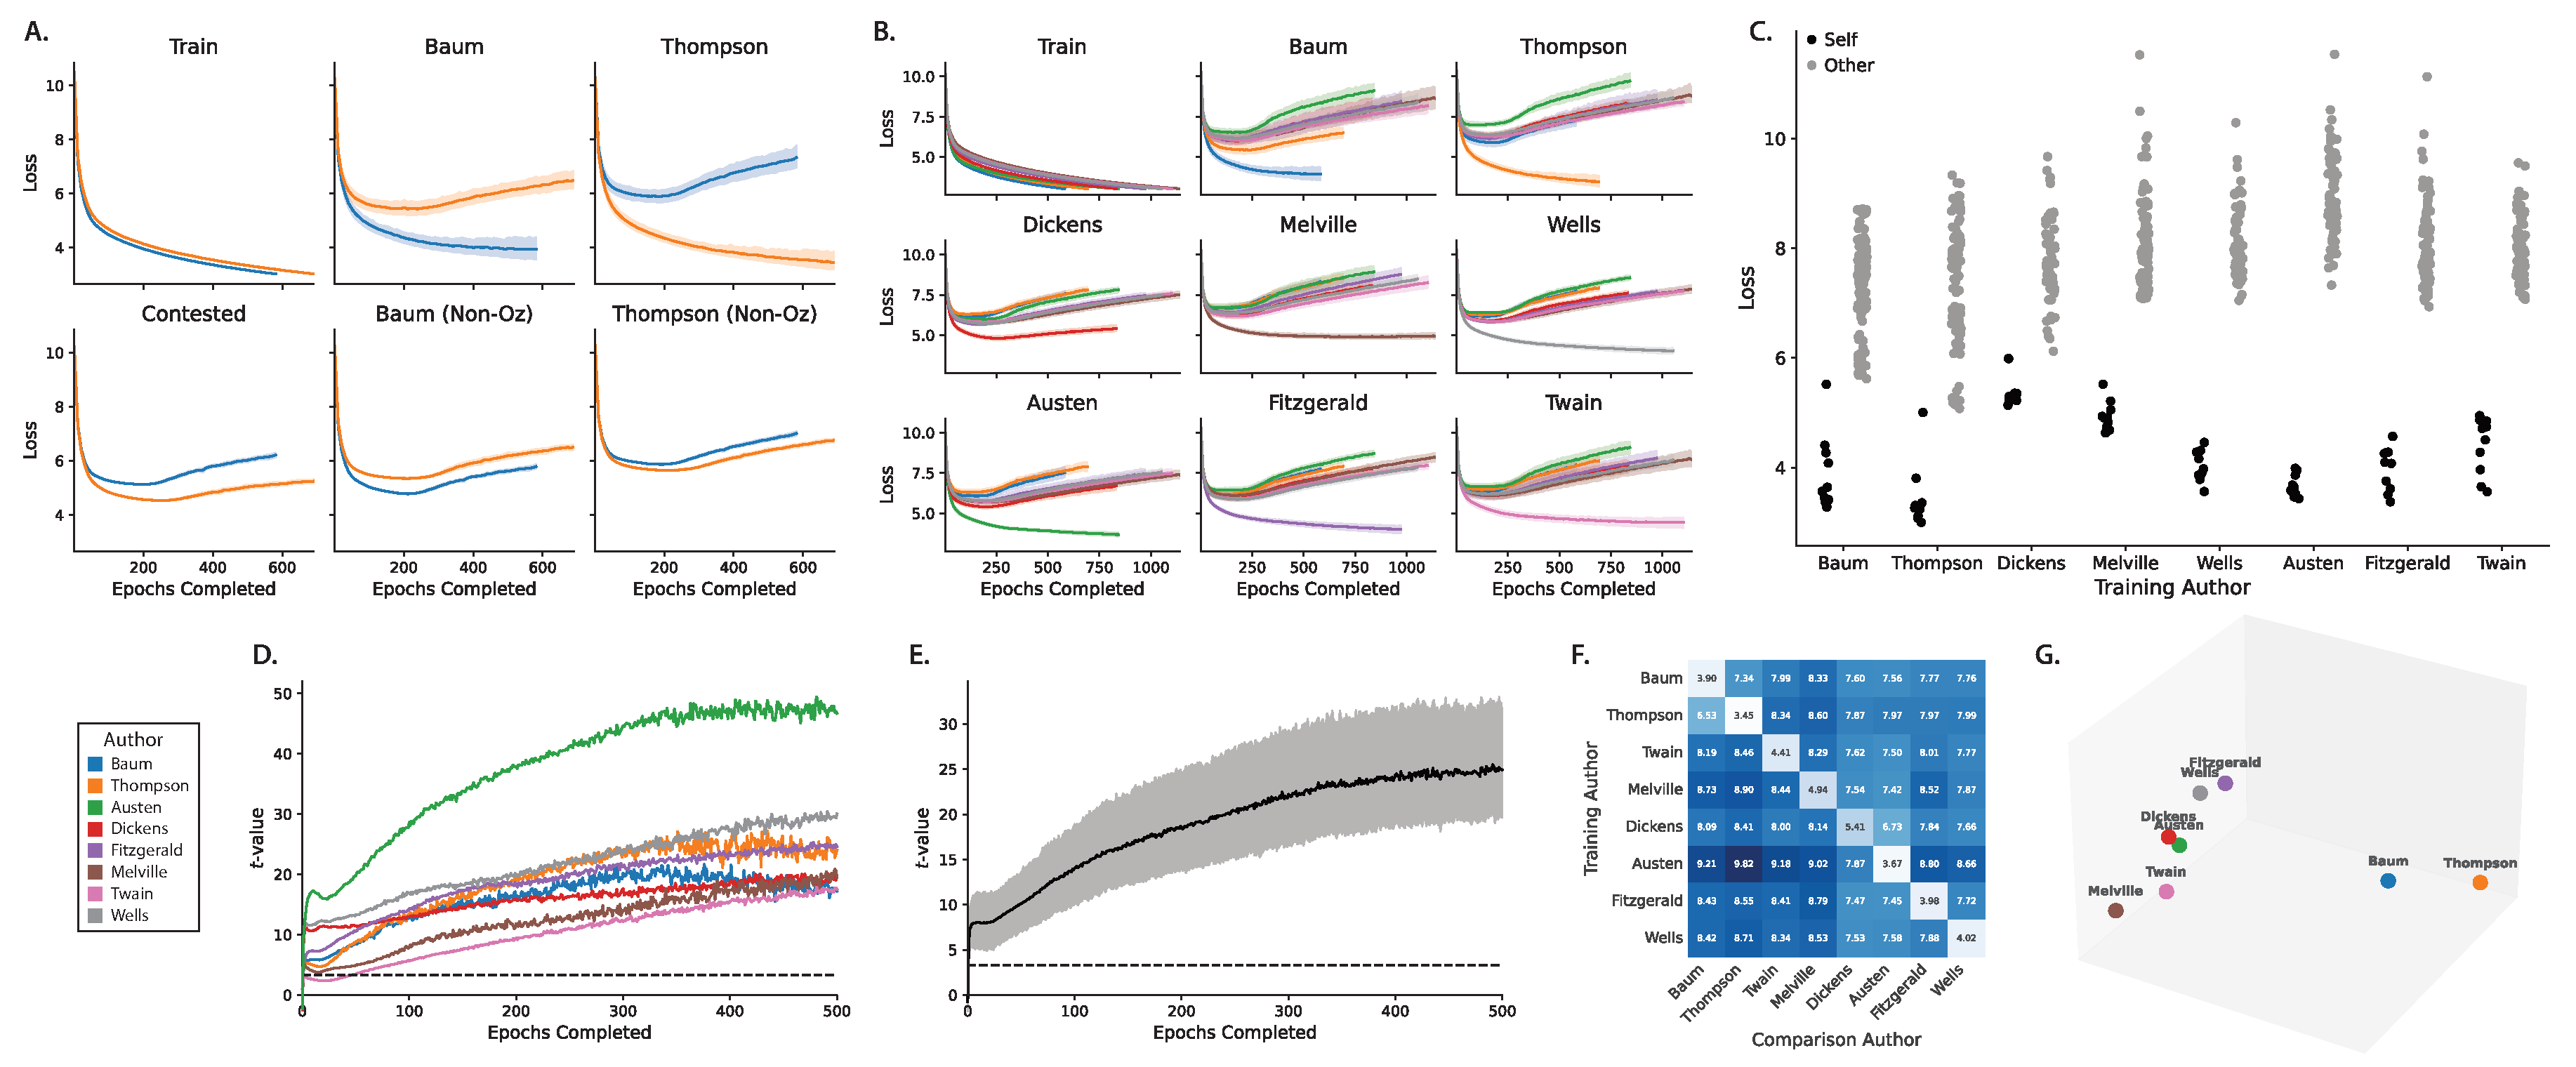
\includegraphics[width=\textwidth]{figs/merged.pdf}
  \caption{\textbf{A.} Average cross-entropy loss on evaluation texts for models trained on Baum and Thompson. Each model is trained with a different random seed; we report the mean cross-entropy loss across 10 random seeds, with error bars indicating a 95\% confidence interval.
\textbf{B.}  Average cross-entropy loss on evaluation texts across all eight authors. Error bars denote 95\% confidence intervals over 10 random seeds.
  \textbf{C.} $t$-test results by author for the first 500 training epochs.
  \textbf{D.} Averaged $t$-test results for the first 500 training epochs.}
  % Training loss is roughly similar for both. Thompson models perform better on Thompson texts, and Baum models on Baum texts. Thompson models also have lower loss on the contested 15th \emph{Oz} book. Error bars denote 95\% confidence intervals over 10 random seeds.
  \label{fig:merged}
\end{figure*}

\subsubsection{Eight-Author Comparison}

We then extend our predictive comparison framework to a broader set of eight
authors. For each author, we compute the predictive loss of the corresponding
model on a held-out book by that author, as well as on one randomly selected
book from each of the other authors. As before, evaluation is based on average
next-token cross-entropy loss computed using a sliding window.

Figure~\ref{fig:merged}B presents the evaluation results across all eight
authors. Training losses are again comparable across models, ensuring a fair
basis for comparison. For each author, we compare the predictive losses of all
models on that author's held-out text. For every author's held-out text, the
model trained on the matching author achieves the lowest loss, indicating a
clear preference for its own author's stylistic patterns. This consistent
alignment provides strong evidence that the GPT-2 models have learned to encode
author-specific stylometric features.

\subsection{$t$-tests}

To validate our findings in the comparison between Baum and Thompson, we
conduct a paired $t$-test on the average cross-entropy losses of the two models
evaluated on the contested 15\textsuperscript{th} \emph{Oz} book. The test
revealed a statistically significant difference in predictive performance,
$t(9) = 20.723, p = 6.6 \times 10^{-9}$. These results provide strong evidence
that the Thompson-trained models predict the contested text more accurately,
aligning with the prevailing literary consensus regarding its authorship.

We also conduct a $t$-test for the eight-author comparison. Specifically, for
each author's model, we perform $t$-tests for (i) the loss values computed by
using the author's models to predict the author's held-out text and (ii) the
loss values computed by using the author's models to predict the other authors'
randomly sampled texts. Table~\ref{tab:author_t_tests} shows the results of the
$t$-tests computed for each author using the final losses.
Figure~\ref{fig:merged}C illustrates the distribution of loss values for each
author's model across self-authored and other-authored texts. These results
demonstrate that the trained GPT-2 models reliably distinguish the stylometric
features of the corresponding author with high statistical significance.

% After training is complete for each of the 8 authors, we perform $t$-tests for (i) the loss values assigned by the author's models to the author's held-out text and (ii) the loss values assigned by the author's models to the other authors' randomly sampled texts. We show the distributions in Figure \ref{fig:stripplot}. Table \ref{tab:author_t_tests} shows the results of the $t$-tests.

\begin{table}[h]
\centering
\begin{tabular}{lccc}
\hline
\textbf{Author} & \textbf{$t$-stat} & \textbf{p-value} & \textbf{df} \\
\hline
Baum        & 16.96 & $5.78 \times 10^{-9}$  & 10.49 \\
Thompson    & 21.50 & $6.84 \times 10^{-12}$ & 13.60 \\
Dickens     & 18.36 & $6.52 \times 10^{-17}$ & 27.36 \\
Melville    & 24.15 & $1.87 \times 10^{-27}$ & 45.15 \\
Wells       & 35.17 & $1.16 \times 10^{-23}$ & 26.33 \\
Austen      & 47.29 & $4.38 \times 10^{-46}$ & 54.75 \\
Fitzgerald  & 26.03 & $2.22 \times 10^{-18}$ & 22.66 \\
Twain       & 20.13 & $9.67 \times 10^{-11}$ & 12.22 \\
\hline
\end{tabular}
% \caption{We show $t$-statistics, p-values, and degrees of freedom for each author, computed from a $t$-test after training is complete for (i) the loss values assigned by the author's models to the author's held-out text and (ii) the loss values assigned by the author's models to the other authors' randomly sampled texts.}
\caption{$t$-test results for each author on final losses}
\label{tab:author_t_tests}
\end{table}

In addition, we perform the same paired $t$-test at each of the first 500
training epochs, comparing losses on the author's own held-out texts to losses
on texts from other authors. Figure~\ref{fig:merged}D shows the $t$-values as
training progresses. For all authors except Twain, the $t$-statistic exceeds
the threshold corresponding to $p < 0.001$ after just one epoch, indicating
rapid acquisition of author-specific stylometry. For Twain, this threshold is
crossed at epoch 47. Figure~\ref{fig:merged}E plots the average $t$-statistic
across all eight authors over training epochs, further illustrating the early
emergence of stylometric differentiation in the models.





\subsection{Classification}

For each author and each random seed, we compute loss on each evaluation text.
The ``predicted'' author is the author of the evaluation text that has the
lowest loss. Under this classification procedure, we have 100\% accuracy.


\subsection{Stylometric Distance}

Predictive comparison suggests a natural notion of distance between authorial
styles -- if the loss of predicting tokens in a work of author $j$ from a model
derived from from the work of author is close to predicting tokens for the work
of author $i$ and vice-versa, one could say that their writing styles are
similar or nearby. Let $L_i(j)$ denote the average loss of a work of author $j$
for a model trained on author $i$ (the $i,j$-entry of the heatmap/average loss
matrix in Figure~\ref{fig:merged}F). Let $\overline{L_i(j)} = L_i(j)-L_i(i)$,
normalizing the entries by subtracting the native author baseline. Then define
the LLM-based {\em stylometric distance}, $d(i,j) =
\frac{1}{2}\left(\overline{L_i(j)} + \overline{L_j(i)}\right)$.
Figure~\ref{fig:merged}G is a visualization of the relative ``distances"
among our author set.

\section*{Conclusions}

In this paper we introduce {\em predictive comparison}, a new LLM-based
relative stylometric measure. It derives from a simple idea, that if an LLM can
be fine-tuned to write like -- i.e., in the style of -- a given author by
training on the work of an author, then the degree to which such a fine-tuned
model can predict another author's work could be a measure of stylistic
similarity. In this paper we show using a small set of authors and their works,
that this thesis is borne out. This in turn suggests a notion of stylometric
distance which we produce. Lastly, this further suggest a literary
authentication tool that would assign an unknown or contested work to the model
which predictive comparison generates the smallest loss. We use this on a
well-known and once contested book in the \emph{Oz} series, confirming what is
now accepted attribution. We believe this new idea could be of use in
considering questions of authorial influence and stylistic evolution.

\section*{Limitations}

The main limitations of this paper are the breadth of experiments as well as
the oft-acknowledged opacity of the LLM. The results in this paper serve as a
proof-of-concept for the idea of using the structure of a bespoke trained LLM
as a stylometric engine. Only a handful of examples have been tested, but the
results on a classic stylometric test are promising. Also, further testing is
needed to understand what kinds of writing features are being picked up by the
LLM.

%\section*{Acknowledgments}

% %This document has been adapted
% by Steven Bethard, Ryan Cotterell and Rui Yan
% from the instructions for earlier ACL and NAACL proceedings, including those for
% ACL 2019 by Douwe Kiela and Ivan Vuli\'{c},
% NAACL 2019 by Stephanie Lukin and Alla Roskovskaya,
% ACL 2018 by Shay Cohen, Kevin Gimpel, and Wei Lu,
% NAACL 2018 by Margaret Mitchell and Stephanie Lukin,
% Bib\TeX{} suggestions for (NA)ACL 2017/2018 from Jason Eisner,
% ACL 2017 by Dan Gildea and Min-Yen Kan,
% NAACL 2017 by Margaret Mitchell,
% ACL 2012 by Maggie Li and Michael White,
% ACL 2010 by Jing-Shin Chang and Philipp Koehn,
% ACL 2008 by Johanna D. Moore, Simone Teufel, James Allan, and Sadaoki Furui,
% ACL 2005 by Hwee Tou Ng and Kemal Oflazer,
% ACL 2002 by Eugene Charniak and Dekang Lin,
% and earlier ACL and EACL formats written by several people, including
% John Chen, Henry S. Thompson and Donald Walker.
% Additional elements were taken from the formatting instructions of the \emph{International Joint Conference on Artificial Intelligence} and the \emph{Conference on Computer Vision and Pattern Recognition}.

% Bibliography entries for the entire Anthology, followed by custom entries
%\bibliography{anthology,custom}
% Custom bibliography entries only
\bibliography{custom}

\clearpage

\newpage


\appendix

\section{Authors, Books, Tokens}
\label{sec:appendixA}

\twocolumn[
\begin{center}
    
\begin{tabular}{@{}ll|ll@{}}
\toprule
\textbf{Charles Dickens} & \textbf{Tokens} & \textbf{Herman Melville} & \textbf{Tokens} \\
\midrule
A Christmas Carol & 38,906 & I and My Chimney & 15,341 \\
Oliver Twist & 216,100 & Bartleby, the Scrivener & 19,112 \\
The Old Curiosity Shop & 285,895 & Israel Potter & 88,570 \\
Bleak House & 471,630 & Omoo & 134,628 \\
Dombey and Son & 482,161 & Mardi, Vol. II & 150,347 \\
David Copperfield & 479,387 & The Confidence-Man & 129,059 \\
A Tale of Two Cities & 181,593 & White Jacket & 190,577 \\
Nicholas Nickleby & 446,457 & Mardi, Vol. I & 132,358 \\
American Notes & 129,214 & Moby-Dick & 285,066 \\
The Pickwick Papers & 432,546 & Typee & 114,239 \\
Great Expectations & 244,897 & & \\
Martin Chuzzlewit & 455,995 & & \\
Little Dorrit & 449,230 & & \\
Hard Times & 142,759 & & \\
\textbf{Total} & \textbf{4,456,770} & \textbf{Total} & \textbf{1,259,297} \\
\bottomrule
\end{tabular}


\vspace{2em}

\begin{tabular}{@{}ll|ll@{}}
\toprule
\textbf{L. Frank Baum} & \textbf{Tokens} & \textbf{Ruth Plumly Thompson} & \textbf{Tokens} \\
\midrule
Ozma of Oz & 52,039 & The Giant Horse of Oz & 51,036 \\
Dorothy and the Wizard in Oz & 53,849 & The Cowardly Lion of Oz & 61,666 \\
Tik-Tok of Oz & 63,781 & Handy Mandy in Oz & 44,778 \\
The Road to Oz & 52,866 & The Gnome King of Oz & 51,687 \\
The Magic of Oz & 51,166 & Grampa in Oz & 55,169 \\
The Patchwork Girl of Oz & 75,703 & Captain Salt in Oz & 61,797 \\
The Wonderful Wizard of Oz & 49,686 & Ozoplaning with the Wizard of Oz & 50,660 \\
The Lost Princess of Oz & 60,418 & The Wishing Horse of Oz & 59,490 \\
The Emerald City of Oz & 70,781 & The Lost King of Oz & 58,105 \\
The Tin Woodman of Oz & 57,338 & The Hungry Tiger of Oz & 53,543 \\
Rinkitink in Oz & 62,241 & The Silver Princess in Oz & 47,964 \\
The Marvelous Land of Oz & 54,733 & Kabumpo in Oz & 62,693 \\
Glinda of Oz & 51,218 & Jack Pumpkinhead of Oz & 49,661 \\
The Scarecrow of Oz & 59,593 & & \\
\textbf{Total} & \textbf{815,412} & \textbf{Total} & \textbf{708,249} \\
\bottomrule
\end{tabular}

\end{center}
]

\clearpage

\newpage

\twocolumn[

\begin{center}
\begin{tabular}{@{}ll|ll@{}}
\toprule
\textbf{Austen} & \textbf{Tokens} & \textbf{Twain} & \textbf{Tokens} \\
\midrule
Sense And Sensibility & 153,718 & Adventures Of Huckleberry Finn & 147,655 \\
Mansfield Park & 201,611 & A Connecticut Yankee In King Arthur'S Court & 150,327 \\
Lady Susan & 29,043 & Roughing It & 208,545 \\
Northanger Abbey & 98,090 & The Innocents Abroad & 246,321 \\
Emma & 207,830 & The Adventures Of Tom Sawyer, Complete & 95,059 \\
Pride And Prejudice & 157,777 & The Prince And The Pauper & 88,409 \\
Persuasion & 106,027 & & \\
\textbf{Total} & \textbf{954,096} & \textbf{Total} & \textbf{936,316} \\
\bottomrule
\end{tabular}

\vspace{2em}

\begin{tabular}{@{}ll|ll@{}}
\toprule
\textbf{Fitzgerald} & \textbf{Tokens} & \textbf{Wells} & \textbf{Tokens} \\
\midrule
The Beautiful And Damned & 168,147 & The Red Room & 4,944 \\
Flappers And Philosophers & 84,707 & The First Men In The Moon & 87,615 \\
This Side Of Paradise & 100,796 & The Island Of Doctor Moreau & 55,967 \\
All The Sad Young Men & 85,411 & The Open Conspiracy & 40,271 \\
Tales Of The Jazz Age & 109,997 & A Modern Utopia & 105,810 \\
The Pat Hobby Stories & 51,069 & The Sleeper Awakes & 98,228 \\
The Great Gatsby & 65,136 & The New Machiavelli & 185,158 \\
Tender Is The Night & 145,925 & The War Of The Worlds & 75,727 \\
& & Tales Of Space And Time & 94,711 \\
& & The Invisible Man: A Grotesque Romance & 65,584 \\
& & The Time Machine & 40,184 \\
& & The World Set Free & 80,518 \\
\textbf{Total} & \textbf{811,188} & \textbf{Total} & \textbf{934,717} \\
\bottomrule
\end{tabular}
\end{center}
]
\end{document}
